\section{Submeasures}\label{appendixA}

\begin{defin}
  Let $\mathcal{A}$ be a boolean algebra and $\mu\colon \mathcal{A} \to [0, \infty)$. The map $\mu$ is called a \textbf{submeasure} if
  \begin{enumerate}[label=\roman*.)]
    \item $\mu(0) = 0$,
    \item $\forall A, B \in \mathcal{A}\colon A \leq B \Rightarrow \mu(A) \leq \mu(B)$,
    \item $\forall A, B \in \mathcal{A}\colon \mu(A \lor B) \leq \mu(A) + \mu(B)$.\qedhere
  \end{enumerate}
\end{defin}

The thesis will assume that every submeasure is a submeasure on the a subalgebra of the power set algebra of a set $X$. This is possible because of the representation Theorem of stone \cite{stone}.

\begin{defin}
  Let $X$ be a set. Then $\Pi(X)$ is the set of all finite partitions of $X$, which means:
  \begin{equation*}
    \Pi(X) := \left\{ \mathcal{A} \subseteq \P(X)\colon (\forall A,B \in \mathcal{A}\colon A \cap B = \emptyset) \: \land \: \bigcup\mathcal{A} = X \: \land \: \left| \mathcal{A} \right| < \infty \right\}.
  \end{equation*}
  Let $\P_1, \P_2 \in \Pi(X)$. $\P_1$ is said to \textbf{refine} $\P_2$ ($\P_2 \preccurlyeq \P_1$) if
  \begin{equation*}
    \forall A \in \P_1\exists B \in \P_2\colon A \subseteq B.
  \end{equation*}
  For every $\P \in \Pi(X)$ define the map $\iota_\P\colon X \to \P$ with
  \begin{equation*}
    \iota_\P\colon x \mapsto \begin{cases}
      &A_1, \: \text{if } x \in A_1, \\
      &A_2, \: \text{if } x \in A_2, \\
      &\vdots \\
      &A_n, \: \text{if } x \in A_n,
    \end{cases}
  \end{equation*}
  where $k = \left|\P\right|$.    
  The set $\Pi(\mathcal{B})$ contains all finite partitions of $X$ but with the additional constraint that they have to be measurable with respect to a submeasure $\mu$ on the boolean algebra of subsets $\mathcal{B}$ of $X$. 
\end{defin}

\begin{defin}
  Let $X$ be a set and let $\mu$ be a submeasure on a subalgebra $\mathcal{B}$ of $\PowS(X)$. Then $\mu$ is called \textbf{diffuse} if
  \begin{equation*}
    \forall \varepsilon\in \R_{>0}\exists \P \in \Pi(\mathcal{B})\forall P \in \P: \mu(P) < \varepsilon.\qedhere
  \end{equation*}
\end{defin}

\begin{defin}
  Let $(P, \leq)$ be a partially ordered set. The set is called directed if for every $p_1, p_2 \in P$ there exists an element $p_3 \in P$ such that
  \begin{equation*}
    p_1 \leq p_3 \: \land \: p_2 \leq p_3.\qedhere
  \end{equation*}
\end{defin}

\begin{thm}\label{thm:algdirected}
  Let $X$ be a set. Then the set $\Pi(X)$ together with the binary operation $\preccurlyeq$ is a directed set.
\end{thm}

\begin{proof}
  Reflexivity and transitivity follow directly from the reflexivity and transitivity of the $\subseteq$ relation.
  Now let $\P_1, \P_2 \in \Pi(X)$. Define $\P_3 := \{ P \cap P' \colon P \in \P_1, \:P' \in \P_2 \}$.
  Since for any two sets $A, B$ it holds that $A \cap B \subseteq A$ and $A \cap B \subseteq B$ it follows that
  \begin{equation*}
    \P_1 \preccurlyeq \P_3 \land \P_2 \preccurlyeq \P_3.\qedhere
  \end{equation*}
\end{proof}

\begin{figure}[ht!]
  \centering
  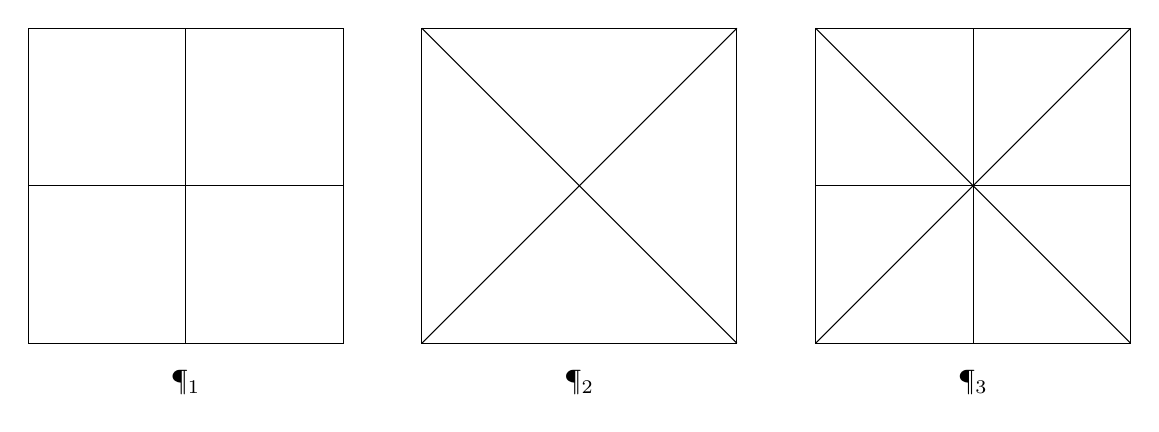
\begin{tikzpicture}
    % Outer square
    \draw (0,0) rectangle (4,4);

    % Vertical and horizontal dividing lines
    \draw (2,0) -- (2,4);
    \draw (0,2) -- (4,2);

    % Outer square
    \draw (5,0) rectangle (9,4);

    % Diagonals
    \draw (5,0) -- (9,4); % Diagonal from bottom-left to top-right
    \draw (5,4) -- (9,0); % Diagonal from top-left to bottom-right
    
    % Outer square
    \draw (10,0) rectangle (14,4);

    % Diagonals
    \draw (10,0) -- (14,4); % Diagonal from bottom-left to top-right
    \draw (10,4) -- (14,0); % Diagonal from top-left to bottom-right
    \draw (10,2) -- (14,2);
    \draw (12,0) -- (12,4);
    
    \node at (2, -0.5) {$\P_1$}; % Label beneath the square
    \node at (7, -0.5) {$\P_2$}; % Label beneath the square
    \node at (12, -0.5) {$\P_3$}; % Label beneath the square
  \end{tikzpicture}
  \caption{Example of 2 partions of the square $\P_1$ and $\P_2$ with common upper bound $\P_3$.}
\end{figure}

\begin{rem}\label{rem:partfinsze}
  If $X$ is an infinite set then $\Pi(X)$ is also infinite.
\end{rem}

\begin{proof}
  Define $\P \subseteq \Pi(X)$ as follows
  \begin{equation*}
    \P := \Big\{ \{ \{x\}, \: X\setminus\{x\}\}\colon \: \forall x \in X \Big\}.
  \end{equation*}
  It is now clear that $\left| \P \right| = \left| X \right|$ and since $\P \subseteq \Pi(X)$ it follows that 
  \begin{equation*}
    \left| X \right| \leq \left| \Pi(X) \right|.
  \end{equation*}
\end{proof}
